% !TEX root = ../main.tex

\subsection{ATLAS Humanoid Robot}

\ldots Humanoid by Boston Dynamics (see Fig. \ref{Fig:AtlasDoorFinals}), \ldots, BDI control modes (aka ``behaviors"), see Fig. \ref{Fig:ControlModeTS}.

\begin{figure}[t]
\centering
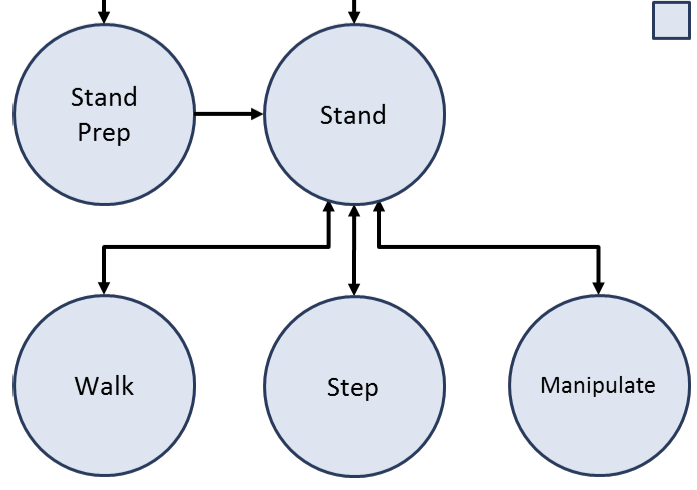
\includegraphics[width=0.99\columnwidth,clip]{./img/control_modes_ts.png}
\caption{\ldots
	\todo[inline, caption = {Create a simple control mode TS figure}]{Placeholder! Create simple control mode TS figure (flat).}
}
\label{Fig:ControlModeTS}
%\vspace{-3 pt}
\end{figure}

\subsection{Team ViGIR's Approach}

\subsubsection{Something}  \ldots Briefly touch on our software approach \cite{TeamViGIR2014JFR}, especially control modes and templates \cite{Alberto2014Humanoids}. Just enough for the ``High-level Control" subsection and the experimental demos to make sense.

\subsubsection{High-level Control} \ldots FlexBE\footnote{\scriptsize{\url{https://github.com/team-vigir/flexbe_behavior_engine}}}
, GUI\footnote{\scriptsize{\url{https://github.com/team-vigir/flexbe_chrome_app}}}
, behaviors and states\footnote{\scriptsize{\url{https://github.com/team-vigir/vigir_behaviors}}}.

Example: Fig. \ref{Fig:FlexBESM} \ldots designed manually by Team ViGIR developers using the FlexBE Editor (graphical user interface).

\begin{figure}[t]
\centering
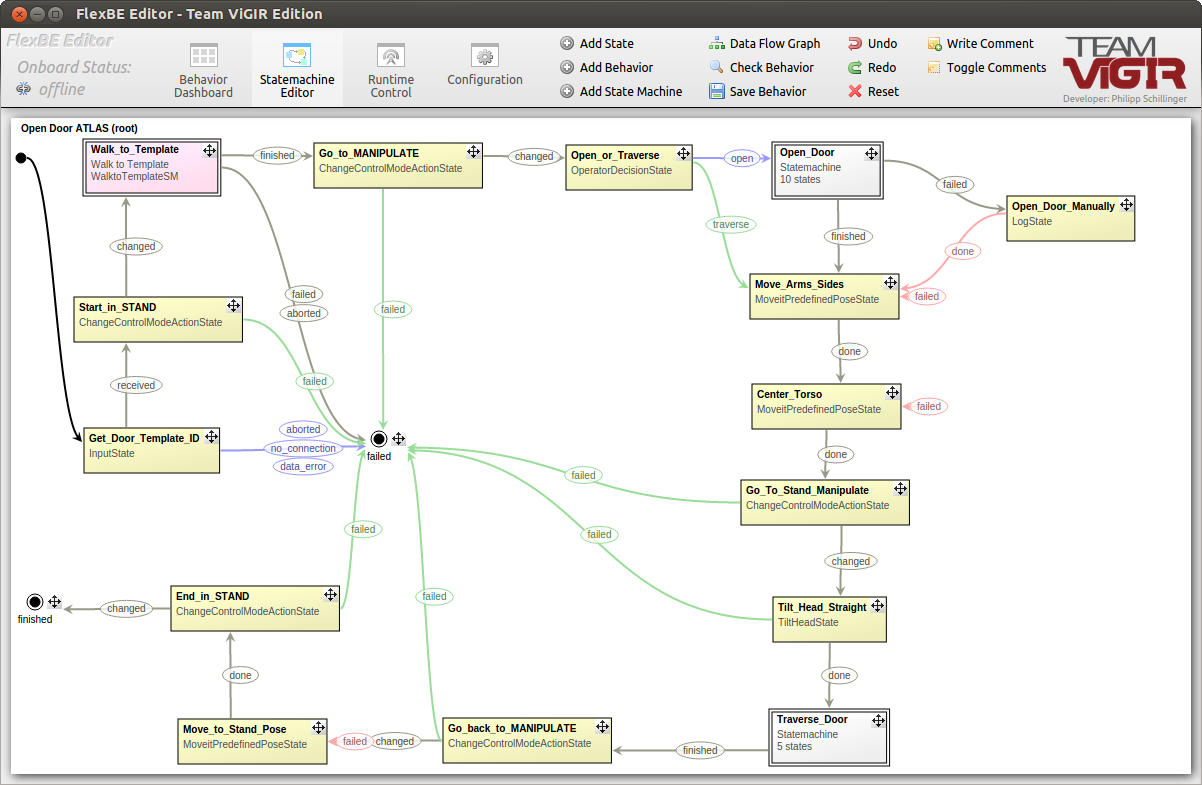
\includegraphics[width=0.99\columnwidth,clip]{./img/behavior_open_door.png}
\caption{A high-level behavior for carrying out the DRC Finals' ``Door" task.
The initial state is indicated by the black arrow originating from the top left.
This state machine has two outcomes, ``finished" (bottom left) and ``failed" (center).
This is a hierarchical state machine. Yellow states are primitives, gray states are state machines, and purple states are other high-level behaviors embedded in this one.
}
\label{Fig:FlexBESM}
\end{figure}

\subsection{Linear Temporal Logic and Reactive LTL Synthesis}

\ldots